\documentclass[5pt,a4paper]{report}
\usepackage[utf8]{inputenc}
\usepackage[francais]{babel}
\usepackage{amsmath}
\usepackage{amsfonts}
\usepackage{amssymb}
\usepackage{graphicx}
\usepackage{listings} 
\usepackage{pdfpages}
\title{Mini-Projet d’Algorithmique}
\author{Julien Defiolles}
\date{Année universitaire 2016-2017}
\begin{document}
	\maketitle
	\part{Partie théorique}
	\section*{Partie 1}
	\subsection*{Question 1.1}
	La complexité d'un algorithme  qui consisterait à énumérer tout les alignements possible serait de $O(d^2)$.
	\subsection*{Question 1.2}
	Supposons que $(x_{^m},y_{^m})\notin M$ et que $x_{^m}$ et $ y_{^m}$ apparaissent dans $M$.
	Alors on peut en déduire que $M$ est aligner sur $m$ c'est à dire qu'il existe une paire $(x_{^m},y_{^m})$. C'est contradictoire donc si $(x_{^m},y_{^m})\notin M$ alors $x_{^m}$ ou $ y_{^m}$ apparait dans $M$.
	\subsection*{Question 1.3}
	\begin{itemize}
		\item test
	\end{itemize}
	\subsection*{Question 1.4}
	$F(m,n) = Min\{F(m-1,n-1),F(m-1,n),F(m,n-1)\}$
	
	\subsection*{Question 1.5}
	$F(i,j) = Min\{F(i-1,j-1),F(i-1,j),F(i,j-1)\}$
	
	\subsection*{Question 1.6}
	Montrons que $F(i,0) = i\delta_{^gap}$ pour tout $i\in \{0,1,...,m\}$ et $F(0,j) = j\delta_{^gap}$ pour tout $j\in \{0,1,...,n\}$\\
	De Base $F(0,0) = 0$ dès que on augmente de 1, $i$ ou $j$, on obtient la valeur du gap, si on augmente $i$ ou $j$ $k$ fois on aura la valeur $k*\delta_{^gap}$ (le seul chemin existant étant de décrémenter $i$ ou $j$).\\ On en déduit que $F(i,0) = i\delta_{^gap}$ pour tout $i\in \{0,1,...,m\}$ et $F(0,j) = j\delta_{^gap}$ pour tout $j\in \{0,1,...,n\}$
	
	\subsection*{Question 1.7}
	\begin{lstlisting}
F : tableau entier de taille m*n

Fonction COUT1(i,j)
	SI F[i,j] != -1
	ALORS
		RETOURNE F[i,j]
	FIN SI
	SI(i = 0 OU j = 0)
	ALORS
		SI (i = 0)
		ALORS
			F[i,j] = j * gap
		SINON
			F[i,j] = i * gap
		FIN SI
		RETOURNE F[i,j]
	FIN SI
	gapi = COUT1(i - 1, j) + gap
	gapj = COUT1(i, j - 1) + gap
	gapij = COUT1(i - 1, j -1) + CoutDiagonale
	F[i,j] = Min(gapi,gapj,gapij)
	RETOURNE F[i,j]
FIN COUT1
	\end{lstlisting}
	Cette algorithme à du $O(n * m)$ en complexité de temps et d'espace, en complexité de 
	temps car il parcourt tout $F$ pour le remplir qui est de taille $n*m$ et d'espace pour $F$.
	
	\subsection*{Question 1.8}
	\begin{lstlisting}
M : Liste contenant l'alignement optimal.

Fonction SOL1(X,Y)
	i = Taille(X)
	j = Taille(Y)
	COUT1(i, j)
	TANT QUE ( i !=0 ET j != 0)
		AJOUTER i,j DANS M
		SI(i != 0) ALORS
			gapi = F[i-1,j]
		FIN SI
		SI(j != 0) ALORS
			gapj = F[i,j-1]
		FIN SI
		SI(i != 0 ET j != 0) ALORS
			gapij = F[i-1,j]
		FIN SI
		SI(Min(gapi, gapj, gapij) = gapi) ALORS
			i = i - 1
			CONTINUER
		FIN SI
		SI(Min(gapi, gapj, gapij) = gapj) ALORS
			j = j - 1
			CONTINUER
		FIN SI
		SI(Min(gapi, gapj, gapij) = gapij) ALORS
			i = i - 1
			j = j - 1
		FIN SI
	FIN TANT QUE
	RETOURNER M
FIN SOL1
	\end{lstlisting}
	Cette algorithme à du $O(n + m)$ en complexité de temps, car on décrémente forcement $i$ ou $j$ ou les deux.\\
	Au final cette approche a pour complexité $O(n * m)$ en temps et en espace.
	
	
	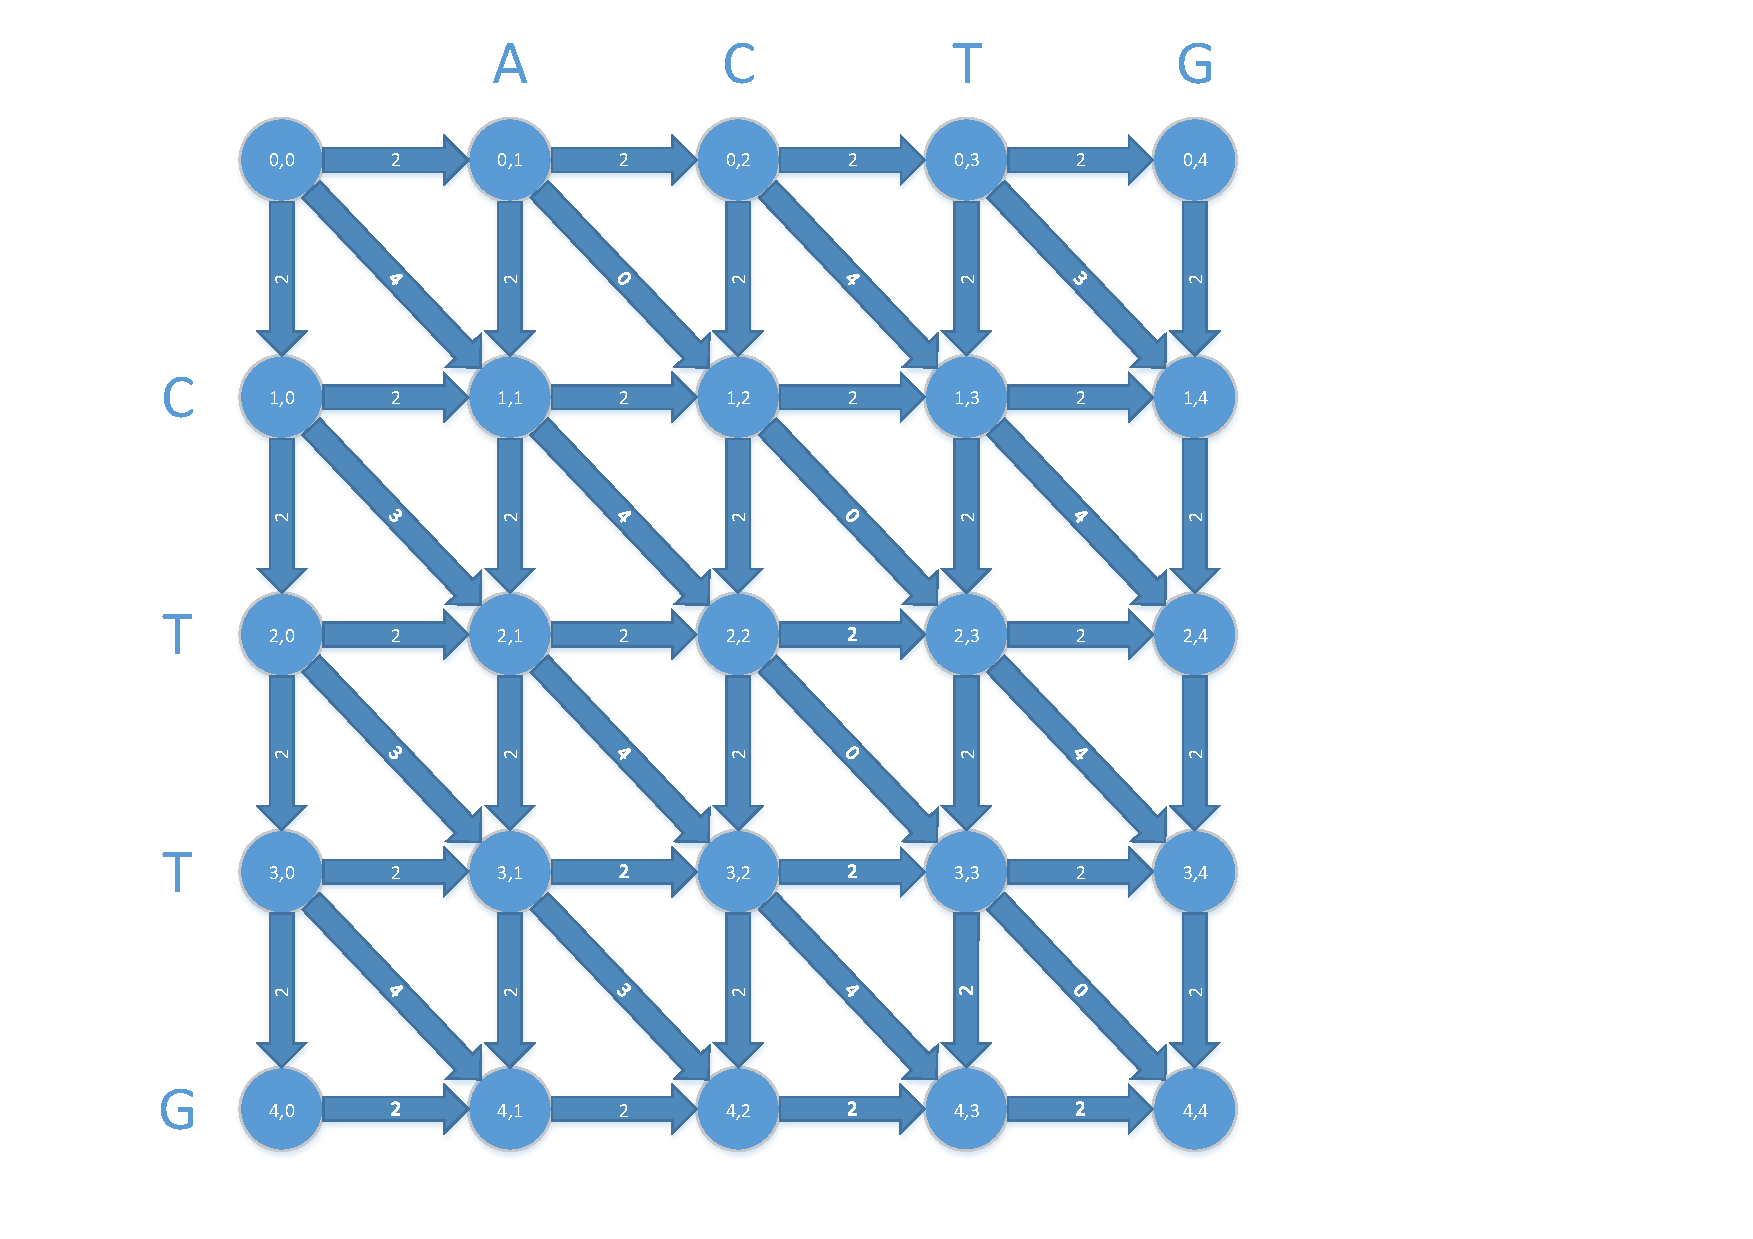
\includepdf[pages=1,pagecommand=\section*{Partie 2}\subsection*{Question 2.1}]{Q2}
	\subsection*{Question 2.2}
	Todo
	\subsection*{Question 2.3} 
	Un algorithme de Dijkstra serait parfait pour calculer le plus court chemin entre $(0,0)$ et $(m,n)$, la complexité de celui-ci est de $O(m*log(n))$.
	\includepdf[pages=7]{Q23}
	Après exécution de l'algorithme de Dijkstra, on voit que le coût minimale de cet alignement est de 4. On trouve l'alignement optimal:\\
	ACT\_G
	\_CTTG
	
	\subsection*{Question 2.4}
	Oui on obtient une meilleure complexité, on a du $O(m*log(n)$ pour cette solution alors qu'à la question 1 on avait du $O(n*m)$.
	
	\section*{Partie 3}
	\subsection*{Question 3.1}
	Pour la partie 1 et 2, on a besoin d'un tableau de taille $n*m$.\\
	Soit $k = max(n,m)$, on peut dire qu'il nous faut au maximum un tableau de taille $k^2$.\\
	Donc pour une mémoire vive de $8$Go soit $8*10^9$o il faut $k = \sqrt(8*10^9) = 89442$.\\
	Et pour une mémoire vive de $32$Go soit $32*10^9$o il faut $k = \sqrt(32*10^9) = 178885$.\\
	Donc on pourra pas avoir d'ADN de plus de 89442 protéines avec 8Go de RAM et de 178885 protéines avec 32Go de RAM.
	
	\subsection*{Question 3.2}
	\begin{lstlisting}
Fonction COUT2(i)
K : Liste entier de taille n
Si i = 0
	Pour j allant de 0 a n
		K[j] = j * gap
	Fin Pour
	Retourner K
Fin Si
KMoins1 = COUT2(i-1)
	Pour Pour j allant de 0 a n
		Si j != 0
			gapj = K[j - 1]
			gapij = KMoins1[j - 1]
		Fin Si
		gapi = KMoins1[j]
		gapi = gapi + gap
		gapj = gapj + gap
		gapij = gapij + CoutDiagonale
		K[j] = min(gapi,gapj,gapij)
	Fin Pour
	Retourner K
Fin COUT2
	\end{lstlisting}
	Cette algorithme à du $O(i * j)$ en complexité de temps et du $O(n)$ d'espace, en complexité de 
	temps car il passe par tout i puis par tout j et d'espace car il stocke 2 tableau de taille $n$.
	
	\subsection*{Question 3.3}
	\begin{lstlisting}
Fonction COUT2Bis(i,j,m)
	K : Liste entier de taille m - j
	Si i = m
		Pour l allant de 0 a m - j
			K[l] = l * gap
		Fin Pour
		Retourner K
	Fin Si
	KMoins1 = COUT2(i,j,m-1)
	Pour i allant de 0 a m - j
		Si l != 0
			gapj = K[l - 1]
			gapij = KMoins1[l - 1]
		Fin Si
		gapi = KMoins1[l]
		gapi = gapi + gap
		gapj = gapj + gap
		gapij = gapij + CoutDiagonale
		K[l] = min(gapi,gapj,gapij)
	Fin Pour
	Retourner K
Fin COUT2
	\end{lstlisting}
	
	\subsection*{Question 3.4}
	La longueur du plus court chemin pour aller à $(i,j)$ est $g(i,j)$, la longueur du plus court chemin pour aller à $(m,n)$ à partir de $(i,j)$ est $h(i,j)$, on en conclue que la longueur du plus court chemin passant par $(i,j)$ est la somme de $h(i,j)$ et de $g(i,j)$.\\
	On peut en déduire que pour calculer le plus court chemin passant par $(i,j)$, il faut calculer $g(i,j)$ et $h(i,j)$ et puis faire la somme des deux.
	
	\subsection*{Question 3.5}
	La complexité spatiale de SOL2 est de $O(m+n)$, car il faut enregistrer le chemin dans L, et dans le pire des cas il passera au moins une fois par tout les i et tout les j.
	L'algorithme utilisé par l'étape 1 est:
	\begin{lstlisting}
i* =  k1
valmin  = COUT2(k1, j)+COUT2BIS(k1, j)
Pour i de k1 + 1 a k2 Faire
	val=COUT2(i, j)+COUT2BIS(i, j)
	Si valmin > val Alors
		valmin = val
		i* =  i
	FinSi
FinPour
	\end{lstlisting}
\part{Partie pratique}

\end{document}
